\documentclass[12pt]{article}
\usepackage[margin=1in]{geometry}
\usepackage{amsmath}
\usepackage{siunitx}
\usepackage{graphicx}
\usepackage{subcaption}
\usepackage{csvsimple}

\setlength{\parskip}{1em}

\begin{document}

\title{DD2424 Deep Learning in Data Science Assignment 1}
\author{Lin Chun Hung, chlin3@kth.se}

\maketitle

\section{Basic Part (Part 1)}
In this exercise, a python version of multi-linear classifier was implemented.
The function for computing the gradients with analytical method was sucessfully implemented.

Unit tests for the function computing the gradient were written. In those unit tests,
I used \texttt{numpy.testing.assert\_allclose} to check if all the elements of two pairs of gradients,
\texttt{gradW} and \texttt{gradb}, computed from the analytical method and the numerical methods are closed.
In the testing assertion, the following equation is element-wise true, otherwise the unit test will fail.

\begin{equation*}
    % absolute(a - b) <= (atol + rtol * absolute(b))
    |a - b| \leq (\texttt{atol} + \texttt{rtol} * |b|)
\end{equation*}
where \texttt{atol} and \texttt{rtol} are the tolerance parameters.

Since the forward difference method is less accurate than the central difference method,
the tolerance parameters are different when comparing them to analytical method.
In the test setting, comparing the analytical method with
the forward difference method is loose while
comparing with the central difference method is tight.
I set \texttt{atol} as \num{1e-7} and \texttt{rtol} as \num{1e-06} for the
forward difference method and set \texttt{atol} as \num{1e-9} and \texttt{rtol} as \num{1e-07}
for the central difference method.

Here is the four parameter sets:
\begin{enumerate}
    \item  \texttt{lambda=0.0, n\_epochs=40, n\_batch=100, eta=0.1}
    \item  \texttt{lambda=0.0, n\_epochs=40, n\_batch=100, eta=0.01}
    \item  \texttt{lambda=0.1, n\_epochs=40, n\_batch=100, eta=0.01}
    \item  \texttt{lambda=1.0, n\_epochs=40, n\_batch=100, eta=0.01}
\end{enumerate}
These four parameter sets are called as parameter set 1, parameter set 2,
and so on in the figures and the table.

The cost functions, the learnt weight matrices and the test accuracies of these four
sets of parameters are persented in figure \ref{fig:cost_fun}, figure \ref{fig:wgt_mat},
and table \ref{table:accuracy} respectively.

We can see that parameter set 1 has a high learning rate when refering to parameter set 2.
The minimization is kind of overshoot and therefore the cost function
value is oscillating and fail to converge.

When increasing the weighting of the regularization term, the learnt weight matrix
becomes more blurred. The regularization limits the total amount of the weighting
values and as the result the contrast of the elements in the weighting matrix is smaller.

% The cost function
\begin{figure}
    \centering
    \begin{subfigure}[b]{0.475\textwidth}
        \centering
        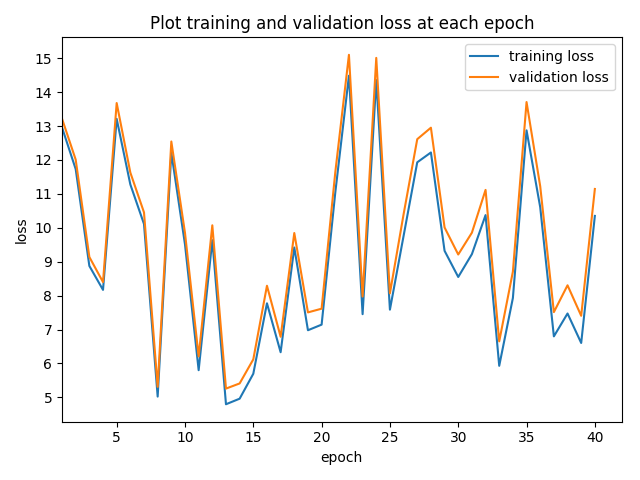
\includegraphics[width=\textwidth]{loss_case1.png}
        \caption[]%
        {{\small Parameter set 1}}
    \end{subfigure}
    \hfill
    \begin{subfigure}[b]{0.475\textwidth}
        \centering
        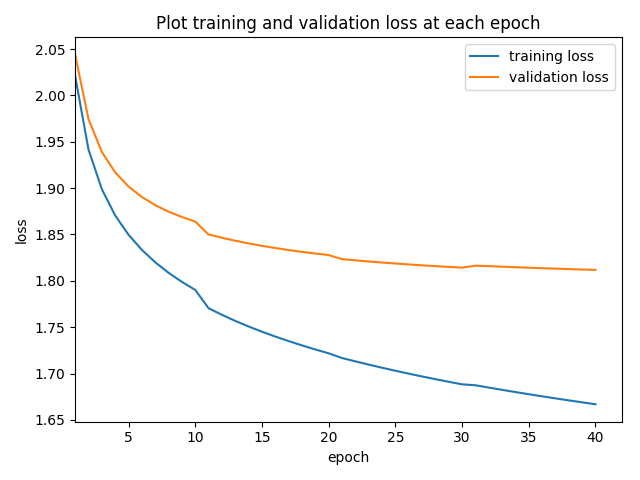
\includegraphics[width=\textwidth]{loss_case2.png}
        \caption[]%
        {{\small Parameter set 2}}
    \end{subfigure}
    \vskip\baselineskip
    \begin{subfigure}[b]{0.475\textwidth}
        \centering
        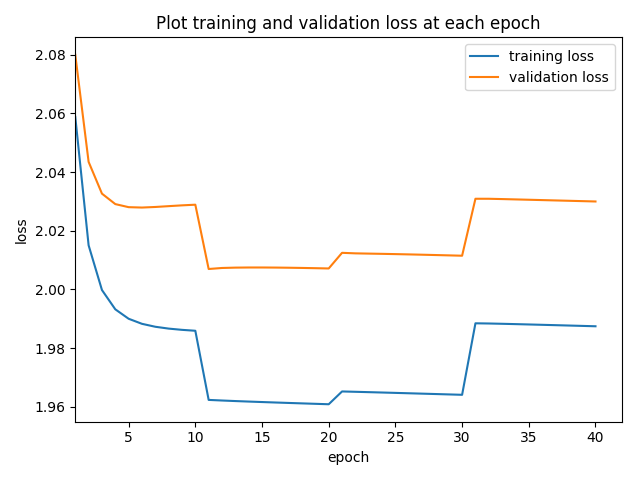
\includegraphics[width=\textwidth]{loss_case3.png}
        \caption[]%
        {{\small Parameter set 3}}
    \end{subfigure}
    \quad
    \begin{subfigure}[b]{0.475\textwidth}
        \centering
        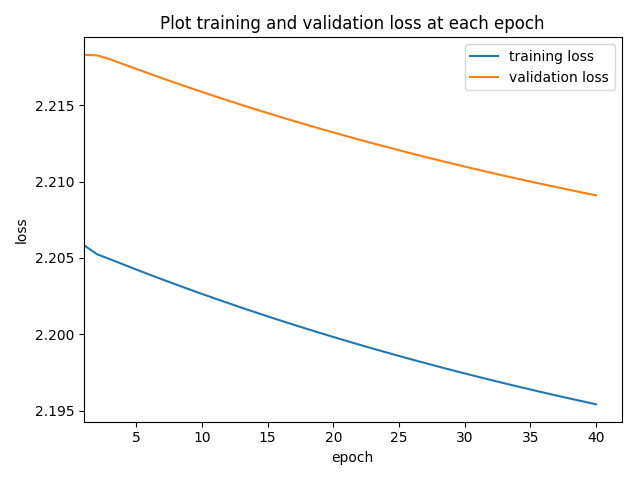
\includegraphics[width=\textwidth]{loss_case4.png}
        \caption[]%
        {{\small Parameter set 4}}
    \end{subfigure}
    \caption[]
    {\small The graph of the training and validation loss computed after each epoch}
    \label{fig:cost_fun}
\end{figure}

% The learnt weight matrix
\begin{figure}
    \centering
    \begin{subfigure}[b]{0.475\textwidth}
        \centering
        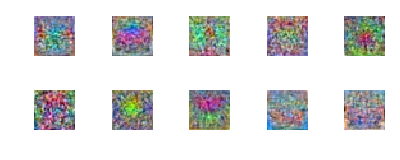
\includegraphics[width=\textwidth]{wgt_case1.png}
        \caption[]%
        {{\small Parameter set 1}}
    \end{subfigure}
    \hfill
    \begin{subfigure}[b]{0.475\textwidth}
        \centering
        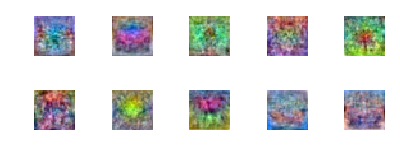
\includegraphics[width=\textwidth]{wgt_case2.png}
        \caption[]%
        {{\small Parameter set 2}}
    \end{subfigure}
    \vskip\baselineskip
    \begin{subfigure}[b]{0.475\textwidth}
        \centering
        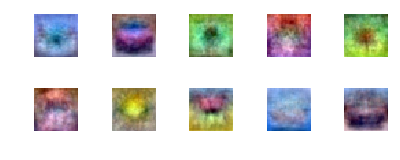
\includegraphics[width=\textwidth]{wgt_case3.png}
        \caption[]%
        {{\small Parameter set 3}}
    \end{subfigure}
    \quad
    \begin{subfigure}[b]{0.475\textwidth}
        \centering
        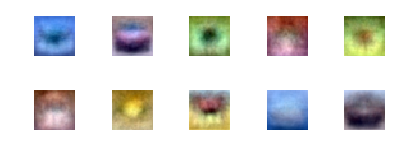
\includegraphics[width=\textwidth]{wgt_case4.png}
        \caption[]%
        {{\small Parameter set 4}}
    \end{subfigure}
    \caption[]
    {\small The Images representing the learnt weight matrix after the completion of training}
    \label{fig:wgt_mat}
\end{figure}

\begin{table}
    \centering
    \csvreader[tabular=|c|c|,respect percent=true,
        table head=\hline Parameter set & Test Accuracy \\\hline,
        late after line = \\\hline]
    {test_accuracy.csv}
    {param_set=\paramset,accuracy=\accuracy}
    {\paramset & \accuracy}
    \caption{The test accuracies of different parameter set}
    \label{table:accuracy}
\end{table}

\section{Bonus Points Part (part 2)}

\subsection{Exercise 2.1}

The best test accuracy is 41.70\%.
The fllowing avenues have been explored and implemented.
\begin{enumerate}
    \item Use all the available training data for training. Retain only 1000 samples
        for validation.
    \item Train for a longer time (\texttt{n\_epoch} $\sim$ 500). Keep the best record
        when the validation cost starts increasing. Stop the iteration when the validation
        cost keep increasing for 5 epochs.
    \item Grid search of the hyper parameters.
    \item Add the linear decay factor. The learing rate will decay with a factor of $\sim 0.9$.
    \item Implement the Xavier initialization.
\end{enumerate}

For the Xavier initialization, it did not have an impact since our original
setting is $\sigma = 0.01$ which is close to the setting in the Xavier initilaization
scheme. The standard deviation used in the Xavier initilaization was:
\begin{equation*}
    \sigma = \frac{1}{\sqrt{n_{in}}} = \frac{1}{\sqrt{3072}} \approx 0.018
\end{equation*}
And therefore it explained why the Xavier initialization did not have an observable
improvement.

To consider which method brought the largest gains, I set the control set as using
the parameter
\texttt{lambda=0.0, n\_epochs=40, n\_batch=100, eta=0.01} and using data\_batch\_1
for training, data\_batch\_2 for validation and test\_batch for testing.
And then I compared it with different tricks.

From the table \ref{table:improve_acc}, we can see that using all training data gave
the largest gain of the test accuracy.
\begin{table}
    \centering
    \csvreader[tabular=|l|c|,respect percent=true,
        table head=\hline Improvement & Test Accuracy \\\hline,
        late after line = \\\hline]
    {improvement.csv}
    {improvements=\improve,test_accuracy=\testAcc}
    {\improve & \testAcc}
    \caption{The test accuracies of different improvement strategies}
    \label{table:improve_acc}
\end{table}

\subsection{Exercise 2.2}
Here is the four parameter sets:
\begin{enumerate}
    \item  \texttt{lambda=0.0, n\_epochs=40, n\_batch=20, eta=0.02, decay=0.9}
    \item  \texttt{lambda=0.0, n\_epochs=40, n\_batch=50, eta=0.005. decay=1.0}
    \item  \texttt{lambda=0.0, n\_epochs=40, n\_batch=100, eta=0.01, decay=1.0}
    \item  \texttt{lambda=0.05, n\_epochs=40, n\_batch=20, eta=0.02, decay=0.9}
    \item  \texttt{lambda=0.1, n\_epochs=40, n\_batch=20, eta=0.02, decay=0.9}
\end{enumerate}
\begin{table}
    \centering
    \csvreader[tabular=|l|c|c|,respect all=true,
        table head=\hline Parameters & SVM Lost test accuracy & Coss-entropy loss test accuracy\\\hline,
        late after line = \\\hline]
    {cmp_ann_svm.csv}
    {params=\params,svm_test_acc=\svm,ann_test_acc=\ann}
    {\params & \svm & \ann}
    \caption{TODO}
\end{table}
\end{document}
